\subsection*{導入：ソフトウェアテストとは何か}
\addcontentsline{toc}{subsection}{導入：ソフトウェアテストとは何か}
\term{ソフトウェアテスト}{Software Testing}とは、通常は無限に近い実行領域から有限個のテストケースを選び、テスト対象システムが期待される振る舞いを提供するかを動的に確認する活動である。この定義には、いくつかの重要な意味が含まれる。

第一に、テストは動的である。つまり、対象を実行して確認する。静的解析、レビュー、形式的証明などは品質向上に重要であるが、この章では主に実行を伴うテストを扱う。

第二に、テストは有限である。すべての入力値、すべての状態、すべての環境を試すことは現実的でない。したがって、テストでは、限られた時間、費用、人員の中で、どのテストケースを選ぶかを決める必要がある。

第三に、テストには期待結果が必要である。実行結果を見ても、それが正しいかどうかを判断できなければテストにならない。期待結果を判断する仕組みがテストオラクルである。

\par\smallskip
\begin{center}
\centering
\IfFileExists{assets/generated_figures/ch05/fig-ch05-02.png}{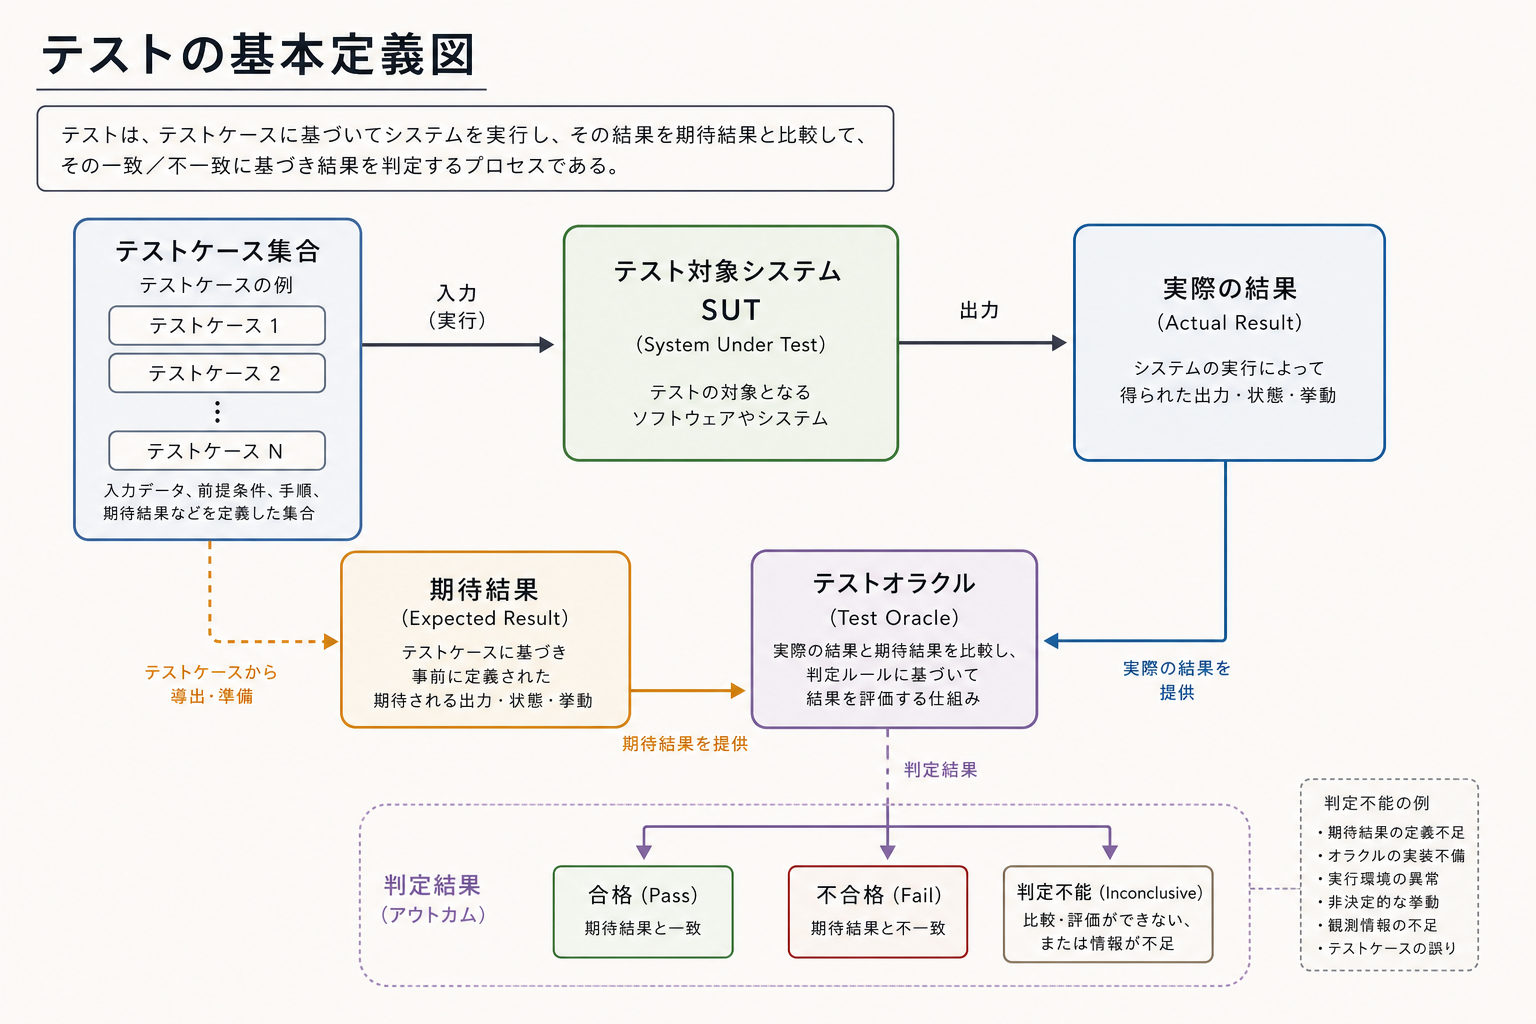
\includegraphics[width=0.96\linewidth]{assets/generated_figures/ch05/fig-ch05-02.png}}{\fbox{\parbox[c][48mm][c]{0.9\linewidth}{\centering 画像生成待ち\\テストの基本定義図}}}
\par\smallskip
\refstepcounter{figure}\label{fig:ch05-02}図 \thefigure: テストの基本定義図
\end{center}
図 \thefigure は、テストの基本定義図を視覚的に整理したものである。
\par\smallskip
